% !TeX spellcheck = zh_CN
\documentclass[aps,pre,12pt,preprint,%
	onecolumn,showpacs,showkeys,nofootinbib]{revtex4-1}
%UnlimitedFonts
	\def\hmmax{0}
	\def\bmmax{0}
%SVG
	\usepackage{svg}
%Tables
	\usepackage{array,booktabs,tabularx,multirow}
	\newcolumntype{C}[1]{>{\hsize=#1\hsize%
		\centering\arraybackslash}X}
%Math&Fonts
	\let\latexointop\ointop
	\usepackage{mathtools,amssymb,bm % basics
		,physics,siunitx,slashed % physics
		,esint,nicefrac,extarrows,mathrsfs % more symbols
		,calligra,romannum,dsfont,fourier-orns % nice fonts
		,eqnarray,resizegather,empheq % more envs
		,relsize,stackengine % utils
	}
%	\usepackage{amsthm}
	\usepackage[scr=esstix]{mathalfa}
	\usepackage[only,sslash]{stmaryrd}
	%DisplaySetup
	\newcommand*\bbox[1]{\fbox{\hspace{1em}\addstackgap[5pt]{#1}\hspace{1em}}}
	\empheqset{box=\bbox}
	\mathtoolsset{showonlyrefs}
%Utils
	%Legacy \oint
	\let\ointop\undefined
	\let\ointop\latexointop
	%Calligra
	\DeclareMathAlphabet{\mathcalligra}{T1}{calligra}{m}{n}
	\DeclareFontShape{T1}{calligra}{m}{n}{<->s*[2.2]callig15}{}
	%CosmeticTweaks
	\newcommand\inlineeqno{\stepcounter{equation}\ (\theequation)}
	\newcommand\scalemath[2]{\scalebox{#1}{\mbox{\ensuremath{\displaystyle #2}}}}
	\newcommand\raisemath[2]{\raisebox{#1\depth}{${#2}$}}
	\newfontfamily\signature{Vladimir Script}
	\newcommand{\newparagraph}{\pagebreak[3]
		\noindent\hfil%
		\raisebox{-4pt}[10pt][10pt]{\leafright~\qquad~\leafleft}%
		\par\nopagebreak%
	}
%CustomCmds
	%Brackets
	\DeclarePairedDelimiter\ave{\langle}{\rangle}
	\DeclarePairedDelimiterX\inprod[2]{\langle}{\rangle}{#1,#2}
	%Basics
	\newcommand{\mbb}[1]{\mathbb{#1}}
	\newcommand{\mrm}[1]{\mathrm{#1}}
	\newcommand{\mcal}[1]{\mathcal{#1}}
	\newcommand{\mscr}[1]{\mathscr{#1}}
	\newcommand{\tup}[1]{\textup{#1}}
	\newcommand{\mop}[1]{\operatorname{#1}}
	%Extras
	\newcommand{\scriptr}{\mathcalligra{r}\,}
	\newcommand{\rvector}{\pmb{\mathcalligra{r}}\,}
	\newcommand{\hodgedual}{\operatorname{\star}}
	\newcommand{\dual}{\ \xlongleftrightarrow{\ \textrm{dual}\ }\ }
	\newcommand{\idty}{\mathds{1}}
	\newcommand{\proj}[1]{\operatorname{%
		proj_{\mathit{#1}}}}
	\newcommand{\propsim}{\mathbin{\ensurestackMath{
		\stackunder[2pt]{\propto}{\sim}
	}}}
	\newcommand{\textbox}[1]{\fbox{#1}}
	\newcommand{\pdd}[1]{\operatorname{\partial_{\mathnormal{#1}}}}
	\newcommand{\cdd}{\operatorname{D}\!}
	\newcommand{\cdv}[1]{\operatorname{%
		\nabla_{\!\mathit{#1}\!}}}
	\newcommand{\ldv}[1]{\operatorname{%
		\mcal{L}_{\!\mathit{#1}\!}}}
	\newcommand{\ric}[1]{\operatorname{%
		Ric}\!\pqty{#1}}
%Hacks
	% physics.sty <texmf-dist/tex/latex/physics/>
	% USER: more spacing around Dirac's middle vert
	\newcommand{\xmiddle}[1]{\mspace{1mu}\middle#1\mspace{1mu}}
	\DeclareDocumentCommand\innerproduct{ s m g }
	{ % Inner product
		\IfBooleanTF{#1}
		{ % No resize
			\IfNoValueTF{#3}
			{\vphantom{#2}\left\langle\smash{#2}\xmiddle\vert\smash{#2}\right\rangle}
			{\vphantom{#2#3}\left\langle\smash{#2}\xmiddle\vert\smash{#3}\right\rangle}
		}
		{ % Auto resize
			\IfNoValueTF{#3}
			{\left\langle{#2}\xmiddle\vert{#2}\right\rangle}
			{\left\langle{#2}\xmiddle\vert{#3}\right\rangle}
		}
	}

%Miscellaneous
%	\newcommand{\tabindent}{\hspace{2em}}
%FourierTransform
	\newcommand{\fourierf}{\mathscr F}
%Atoms
	\newcommand{\CoAtom}{\textsuperscript{\tup{57}}\tup{Co}}
	\newcommand{\FeAtom}{\textsuperscript{\tup{57}}\tup{Fe}}
	\newcommand{\FeAlpha}{$\alpha$--\tup{Fe}}
	\newcommand{\NaSample}{硝普酸钠}
\begin{document}
%Basic Data
	\title{%
	\texstringonly{\hfil\\[2\baselineskip]}
	\sf\LARGE%
		利用穆斯堡尔效应测定超精细结构%
	\texstringonly{\vspace{3ex}}}
	\author{\fangsong\large%
		Bryan%
	\vspace{2mm}}
	\affiliation{\it%
		北京大学物理学院~~学号:\normalfont 1500066666\,}
	\date{\today}
	\keywords{穆斯堡尔效应\ 核能级\ 超精细结构}
	\email{masked_email_please_contact@github.com}

\begin{abstract}
\vspace{10mm}
\begin{spacing}{1.5}\normalsize
\setlength{\parskip}{.3\baselineskip}
%	200—300字,
%	说明用什么方法做了什么事,
%	由此得到什么结果和结论,
%	有何意义.
%	不用缩略词,不用第一人称.
%%%%%%%%%%%%%%%%%%%%%%%%%%%%%%%%
%	实验首先得到了掺有 的 \sHIIO 样品中质子的核磁共振信号,由此验证了核磁共振现象;并在此基础上考察了不同实验条件对核磁共振信号的影响。
%	
%	在此基础上,实验中利用\specWaterPlus 样品质子共振信号和质子回旋频率的参考值对永久磁铁的磁场进行了校准;并进一步利用校准后的磁场测定了氟核的$g$因子。
%	此外,通过估测信号的半宽度$\Delta\omega$, 估测了聚四氟乙烯中氟核的横向弛豫时间;最后观察并比较了纯水与\specWaterPlus 共振信号的差异。
	本实验以 \tup{Pd} 衬底的 \CoAtom 为放射源,获得了 \FeAlpha 与\NaSample 作为吸收体时的穆斯堡尔谱,由此验证了穆斯堡尔效应。
	
	在此基础上,利用穆斯堡尔谱线的尖锐特性,通过对吸收谱的定量分析,测定了 \FeAtom 核能级的塞曼分裂、同质异能移位和电四极分裂等超精细结构;初步了解了穆斯堡尔效应在高分辨探测中的应用。
\end{spacing}
\end{abstract}

\maketitle
\thispagestyle{titlepagestyle}

%	\item 课程实验报告应假定读者既不是已知全部实验细节的指导教师,也不是缺少专业知识的公众,而是同领域的实验研究者,或审稿人. 不能要求读者要在读过课程讲义后才能读懂课程实验报告.
%	\item 公式、图和表要分别用阿拉伯数字编列序号. 公式和图表要达到可发表的质量.
%	\item 凡不是自己独立思考得到的内容都应该引参考文献. 不能大段引用同一参考文献. 对复杂问题,应该优先考虑引用参考文献得到结果. 对简单一些的问题才鼓励独立思考.
%	\item 较长的推导和说明可以作为附件提交,不占用报告篇幅.
%	\item 思考题不是报告的组成部分. 应另起一页附在报告的最后.
\section{引言}
%%	研究论文引言一般包含以下内容:
%%	(1)所研究领域背景和现状;
%%	(2)有待研究的问题;
%%	(3)本研究的目的、主要内容和结果;
%%	(4)结果的意义.\par
%%	在写实验报告的引言时,同学可以假想自己是第一个做类似研究的人.\par
%%	引言一定要切合报告正文,不能漫无目的地介绍背景. 要快速地将读者引导到报告主题上,并作较深入的讨论.\par
%%	引言篇幅可以在较大范围内变化,但最长不应超过报告文字篇幅的1/3.\par
%%	引言撰写可以参考实验讲义,可以复述,但不能复制讲义上的任何一句话.\par
%%%%%%%%%%%%%%%%%%%%%%%%%%%%%%%
\vspace{-1ex}
	$\gamma$光子由于其能量较高,与自由原子核相互作用时导致原子核有显著的反冲;这使得$\gamma$射线能量相对于核能级差出现移动,从而难以实现共振吸收。
	
	直到1957年,德国物理学家穆斯堡尔(R.~L.~Mössbauer)在博士研究期间发现,
	固体中的 \textsuperscript{191}\tup{Ir} 核在$\gamma$射线散射过程中有一定概率不发生反冲,从而出现共振吸收;此即穆斯堡尔效应。其工作 \cite{mossbauer1958kernresonanzfluoreszenz} 于1958年发表,这是最早观测到的$\gamma$射线共振散射现象;该发现于1961年获诺贝尔物理学奖。
	
	穆斯堡尔谱线非常窄,可用于测量十分微小的能量差。例如,著名的Pound–Rebka实验即在穆斯堡尔效应发现后的1959年实现,其利用安放在哈佛Jefferson实验室楼顶与地面之间的一对$\gamma$射线发射、吸收体精确地测得了光子的引力红移\supercite{pound1959gravitational}。与此类似,自然可由穆斯堡尔效应测定吸收体原子的超精细结构;本实验即利用多普勒效应控制入射的无反冲$\gamma$射线能量在小范围内变化,从而分辨并研究了几种典型的核能级超精细结构。
\vspace{-2ex}
\section{理论}
\vspace{-1ex}
\setlength{\jot}{0pt}
	一般来说,共振吸收截面与谱线均为Lorentz线型,其自然线宽:
	\begin{equation}
		\Gamma \sim \frac{\hbar}{\tau}
	\end{equation}
	其中$\tau$为能级寿命。对 \FeAtom 的$E_0 = \SI{14.4}{\keV}$激发态而言,$\tau\sim\SI{.14}{\us}$, 导致$\Gamma\approx\SI{4.9e-9}{\eV}$的尖锐谱线。
	
	而相应地,$\gamma$光子造成的核反冲:
	\begin{equation}
		E_R = \frac{p^2}{2m_N} \approx \frac{E_0^2}{2m_N c^2}
	\end{equation}
	给出$E_R \approx \SI{2e-3}{\eV} \gg \Gamma$, $E_0 \pm E_R$谱线显著分离,难以实现共振吸收。
\clearpage
	
	此外,虽说室温下的多普勒展宽$D\sim\SI{2e-2}{\eV} \gg \Gamma$, 看似有助于共振吸收,但此时相对于原先仅有$\sim\Gamma/D$比率的光子可被吸收,即有效吸收界面被$\Gamma/D\sim\num{2.5e-7}$因子显著压低,实际无助于共振吸收。
	
	\newparagraph
	不过,当原子嵌于晶格中时,其运动规律由固体整体波函数描述:
	\begin{equation}
		\ket{\Psi}
		= \ket{\Psi_A} \otimes \ket{\Psi_B}
			\otimes \cdots
		= \ket{\Psi_A} \otimes \ket{\Psi_{\overline{A}}}
	\end{equation}
	这里$A,B,\dots$标记固体中的各原子,非$A$的原子一并标记为$\overline{A}$. 
	
	设$A$原子与高能$\gamma$光子作用,传递动量$p_0$, 则其波函数的变化规律与经典情形类似,可视为动量空间的平移:
	\begin{equation}
		\braket{p}{\Psi'_A} = \braket{p-p_0}{\Psi_A}
	\end{equation}
	由此得到整体波函数:$\ket{\Psi'} = \ket{\Psi'_A}\otimes\ket{\Psi_B}$, 此时$\ket{\Psi'}$不再是能量本征态,平均反冲能:
	\begin{equation}
		\mel{\Psi'}{\hat{H} - E_0}{\Psi'}
		= E_R,\quad
		E_0 = \mel{\Psi}{\hat{H}}{\Psi}
	\end{equation}
	
	然而,测定固体的吸收、发射谱,本质上正是对固体能量的观测;这一观测导致固体波函数坍缩至某一能量本征态,其中有一定概率回到初态,此即对应无反冲情形。无反冲分数可由终态与初态的交叠加以刻画:$f = \abs{\braket{\Psi}{\Psi'}}^2 = \abs{\braket{\Psi_A}{\Psi'_A}}^2$. 这便是穆斯堡尔效应的基本图像。
\restorejot
\pagebreak
\subsection*{\large 核能级的超精细结构}
	\begin{figure}[!ht]
	\centering
	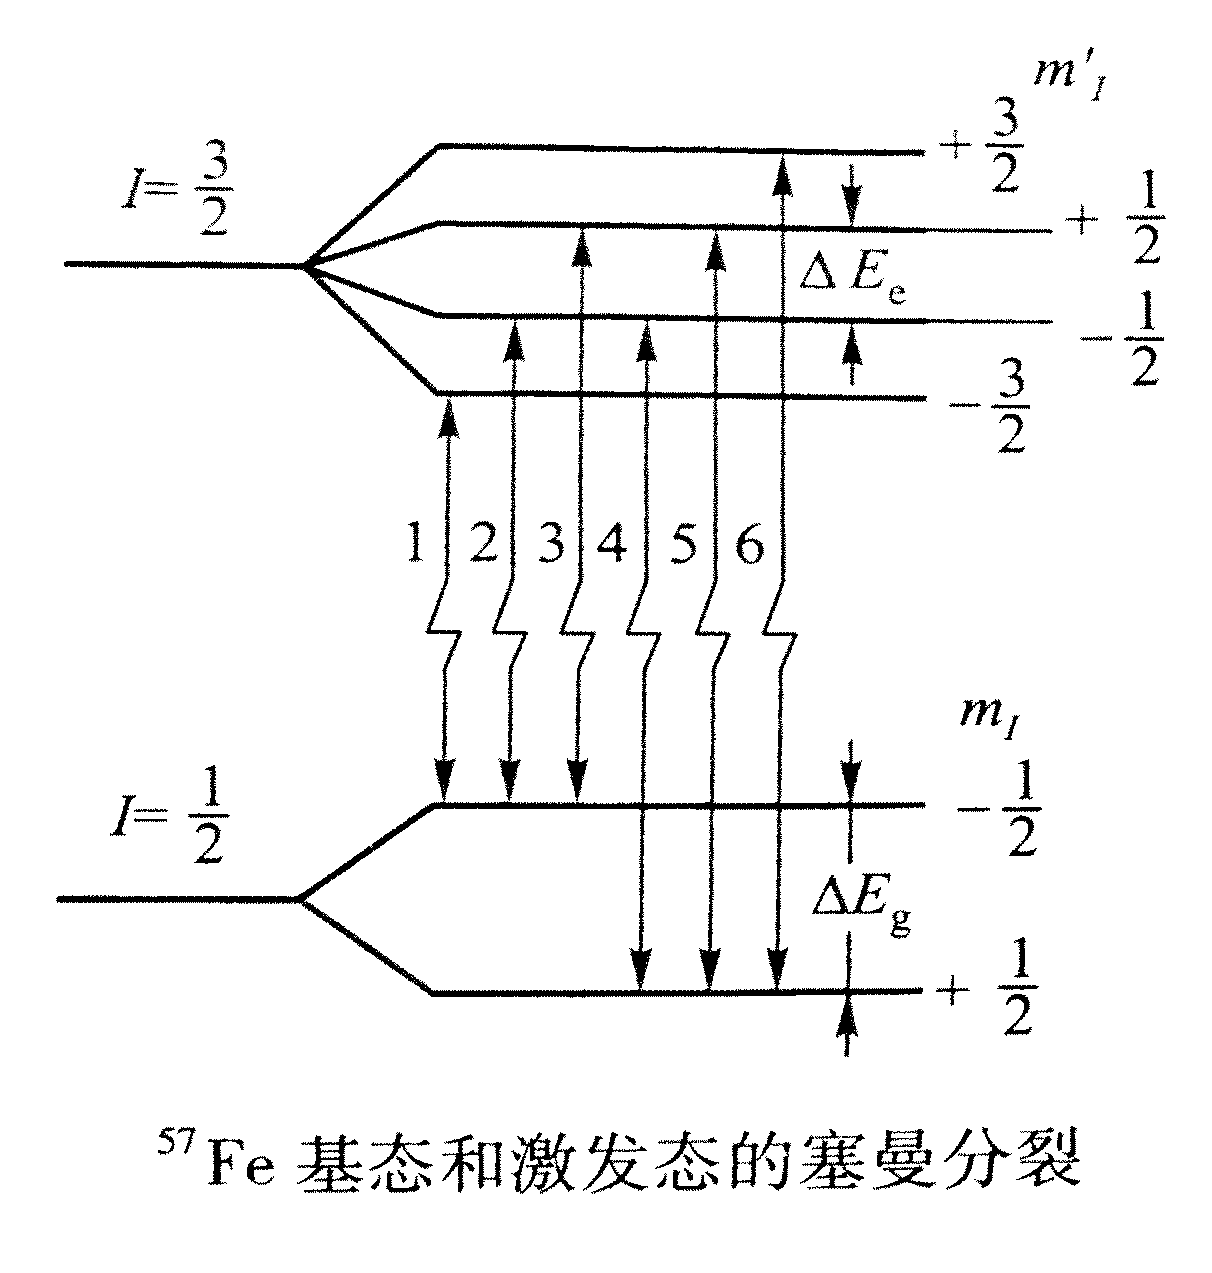
\includegraphics[height=.5\linewidth]{img/2-5-8.png}
	\quad
	\raisebox{1.6ex}{
		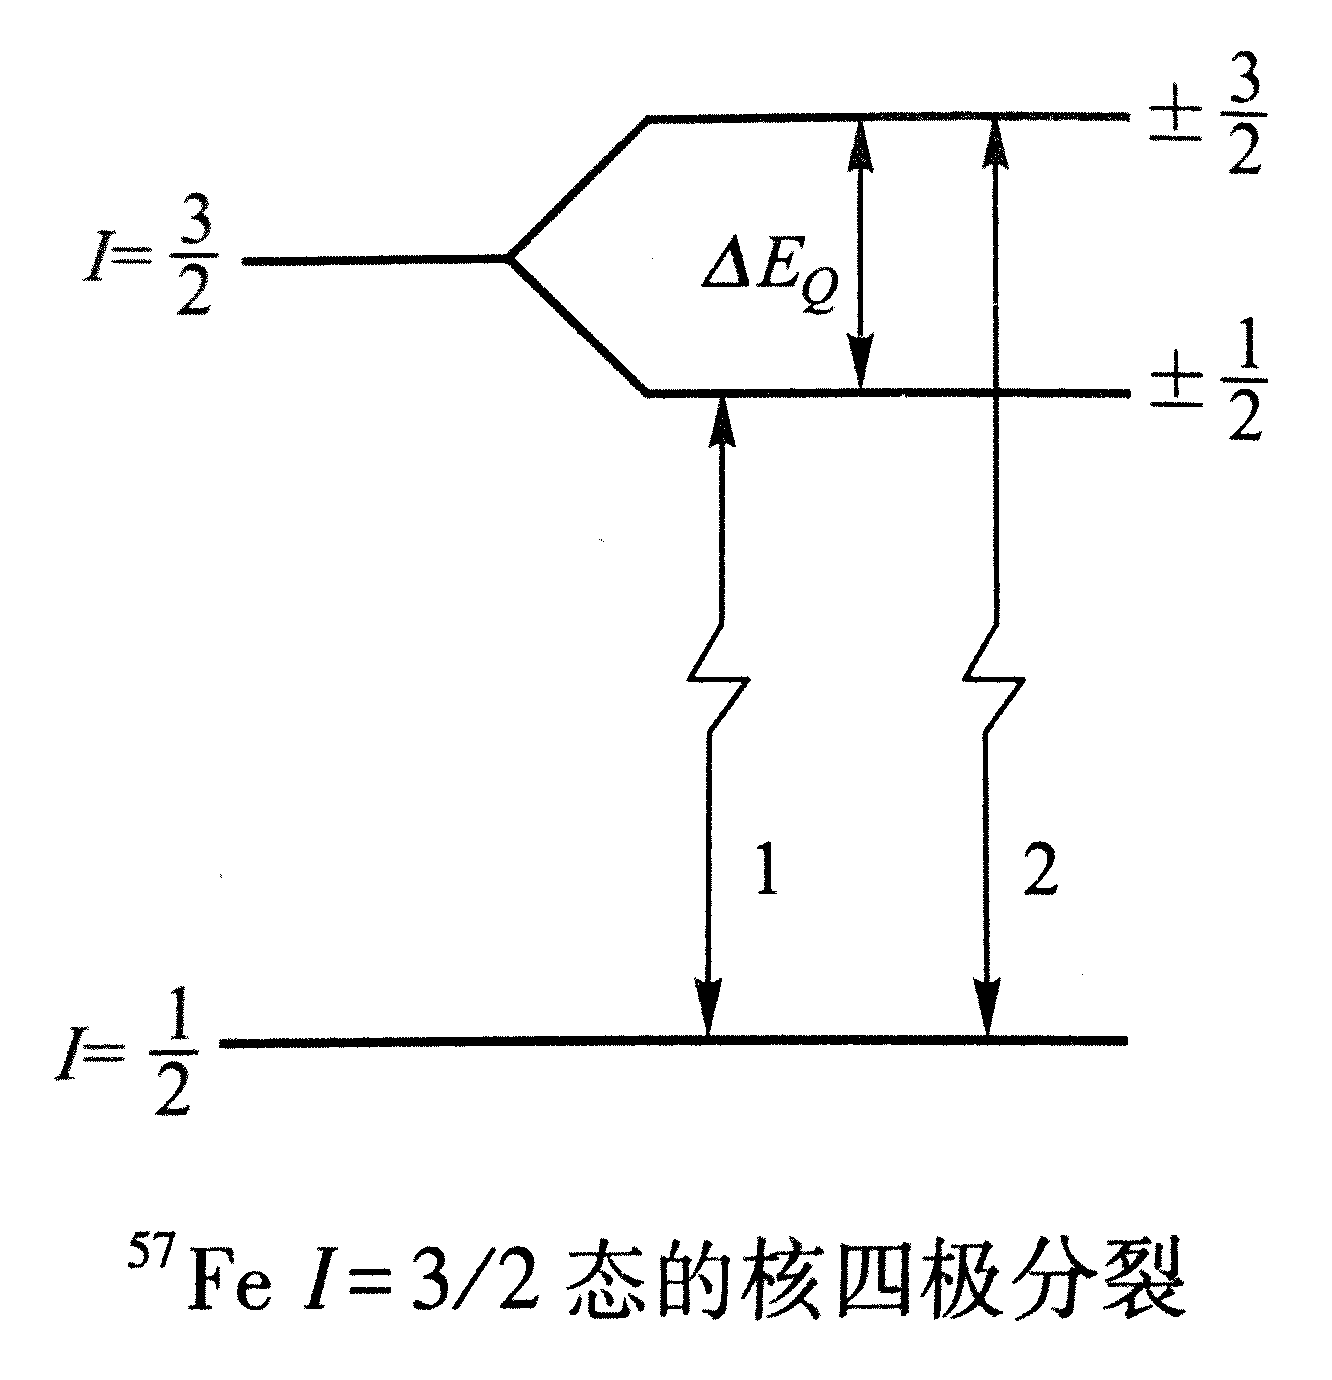
\includegraphics[height=.4\linewidth]{img/2-5-6.png}
	}
	\caption[能级分裂示意图]{%
		\FeAtom 能级分裂示意图,摘自 \cite{textbook}. \\[.5ex]
		图中已标明选择定则容许的$\gamma$跃迁。
	}\vspace{1ex}
	\end{figure}
	如前所述,利用穆斯堡尔效应,可以精确地测定原子核超精细结构;具体有:
	\begin{enumerate}
	\item \textbf{核塞曼分裂:}固体内部磁场$B$与原子核磁矩相互作用导致的塞曼分裂:
	\begin{equation}
		\Delta E = g\mu_N B
	\end{equation}
	其中$\mu_N = \frac{e\hbar}{2m_p}$. 对 \FeAtom 而言,如图所示,这将导致6条相近的谱线。
	\item \textbf{电四极矩分裂:}核电荷分布不均匀导致的能级劈裂:
	\begin{equation}
		\Delta E_Q = \frac{eQ\cdot eq}{2}
	\end{equation}
	其中$eq$对应电场梯度主分量,$eQ$对应电四极矩主分量。对 \FeAtom 而言,如图所示,这将导致2条相近的谱线。
	\item \textbf{同质异能移位:}核外s电子因隧穿效应致其在核内有一定概率分布,又核激发时半径有一定变化,导致能量变化,此即同质异能移位。放射源和吸收体通常有大小不同的同质异能移位,故实际讨论和测量的同质异能移位为不同两者之相对值。
	\end{enumerate}
\FloatBarrier
%%%%%%%%%%%%%%%%%%%%%
\section{实验装置}
\vspace{-1\baselineskip}
%%	在此部分需要将实验条件交待清楚到别人能重复你的实验结果的程度. 此外,还需表明你已尽了最大努力来提高实验精度和结果的可靠性. 简单的不确定度估计可以在此节给出,复杂一些的可以放到分析讨论部分.\par
%%	实验条件不仅是指直接影响实验结果的实验参量,而且还包括影响实验质量和可靠性的因素,如室温、空气湿度、基真空、原材料纯度等.\par
%%	作为教学实验报告,此节写详细一点没有坏处.\par
%%	成段有叙述,必要才分节。
%%%%%%%%%%%%%%%%%%%%%%%%%%%%%%%
	\begin{figure}[!ht]
	\centering
	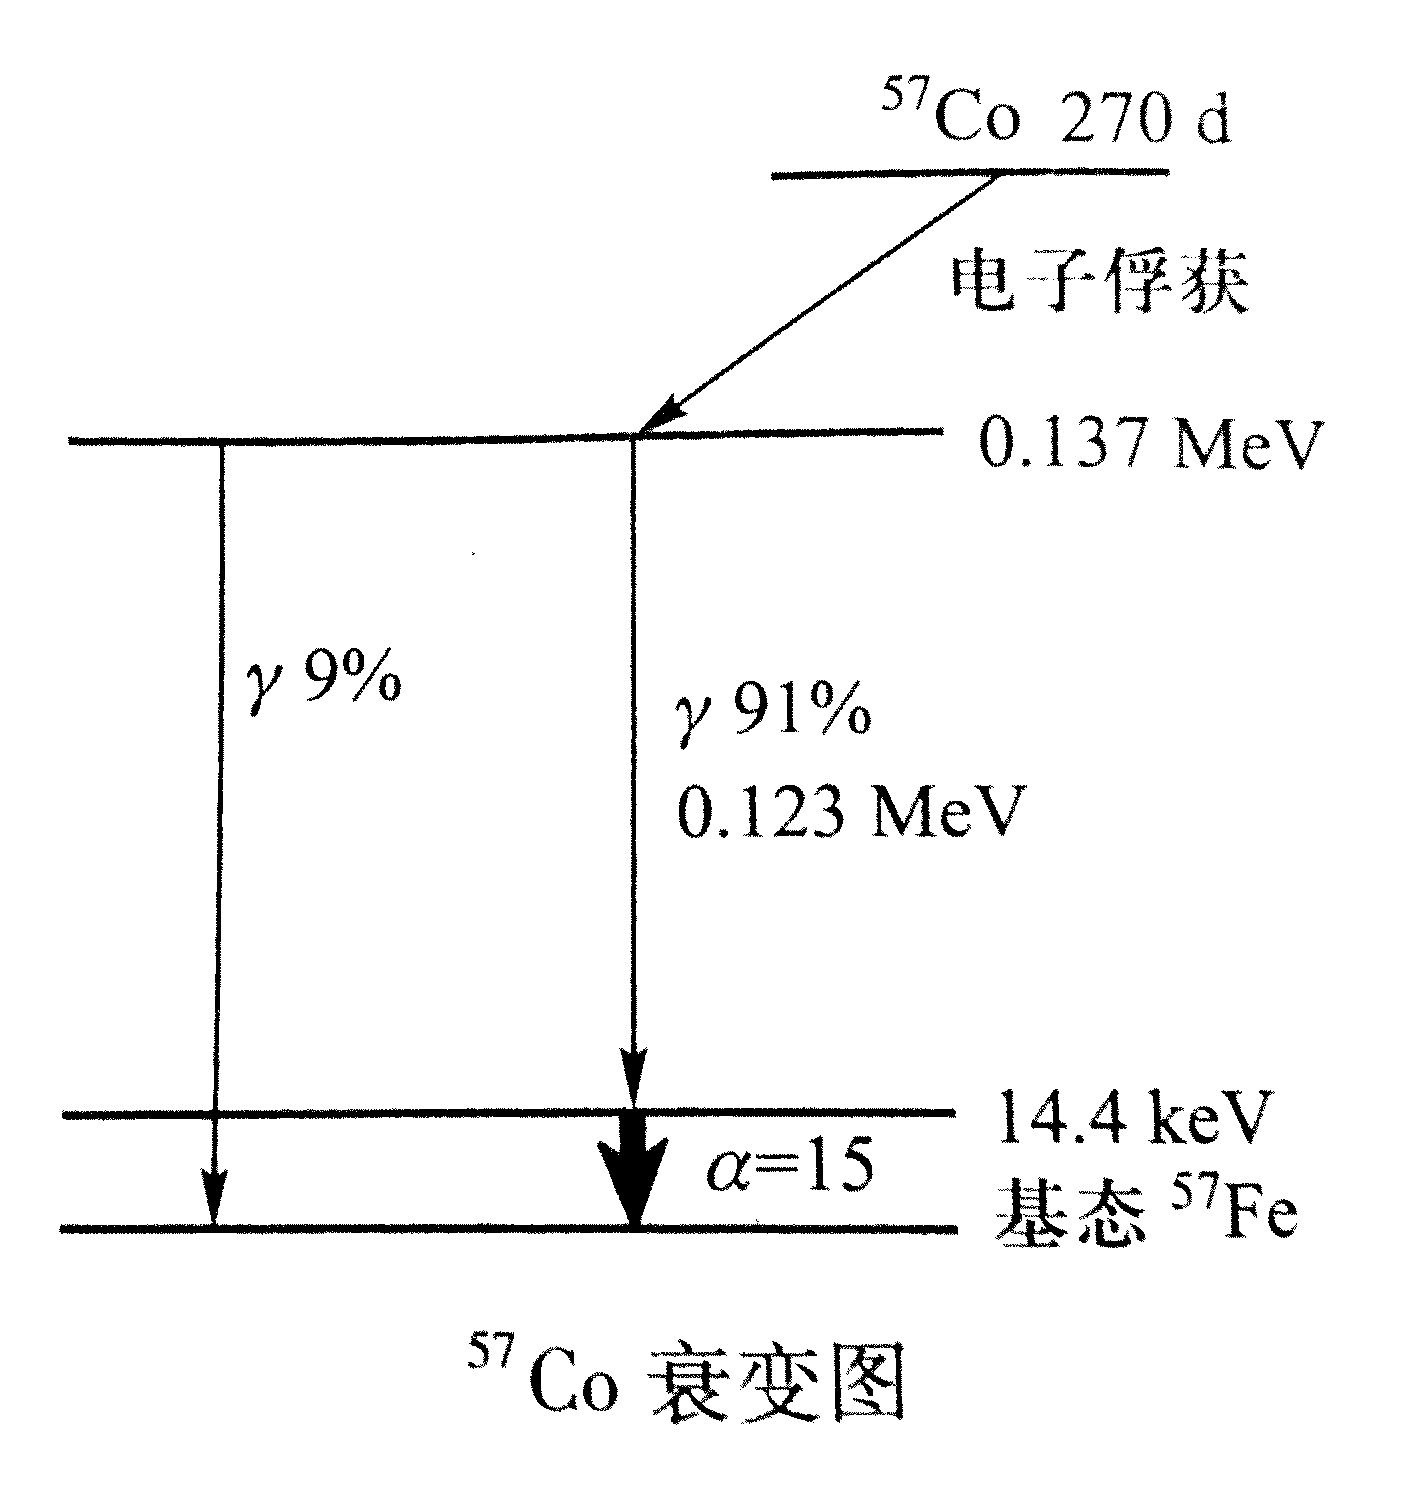
\includegraphics[width=.4\linewidth]{img/decay.png}
	\caption{本实验利用 \FeAtom 退激发射的 \SI{14.4}{\keV} $\gamma$光子。选自 \cite{textbook}. }
%	\begin{explain}
%		NULL
%	\end{explain}
	\end{figure}
	
	本实验采用Pd衬底的 \CoAtom 为$\gamma$源,采用电磁驱动使穆斯堡尔源以 \SI{10}{\Hz} 频率水平往返匀加速运动,利用多普勒效应周期性地、线性地调制$\gamma$射线能量。
	
	采集信号的多道分析器具有脉冲幅度分析(PHA)和多度定标(MCS)两种功能,PHA用以选取实验所需 \SI{14.4}{\keV} 射线,MCS 用以探测穆斯堡尔谱。多度定标模式将不同时刻的脉冲送入不同道址,由于放射源的速度与扫描周期同步变化,故不同道址实际对应于放射源的不同速度。
	
	程序上,通过比较多道分析器信号,反馈调节驱动线圈以保证驱动与输入信号严格同步,从而与多道分析器接收端的扫描同步。$\gamma$射线的探测采用 NaI(Tl) 闪烁体探测器。具体实验装置示意如下。
	
	\begin{figure}[!ht]
	\centering
	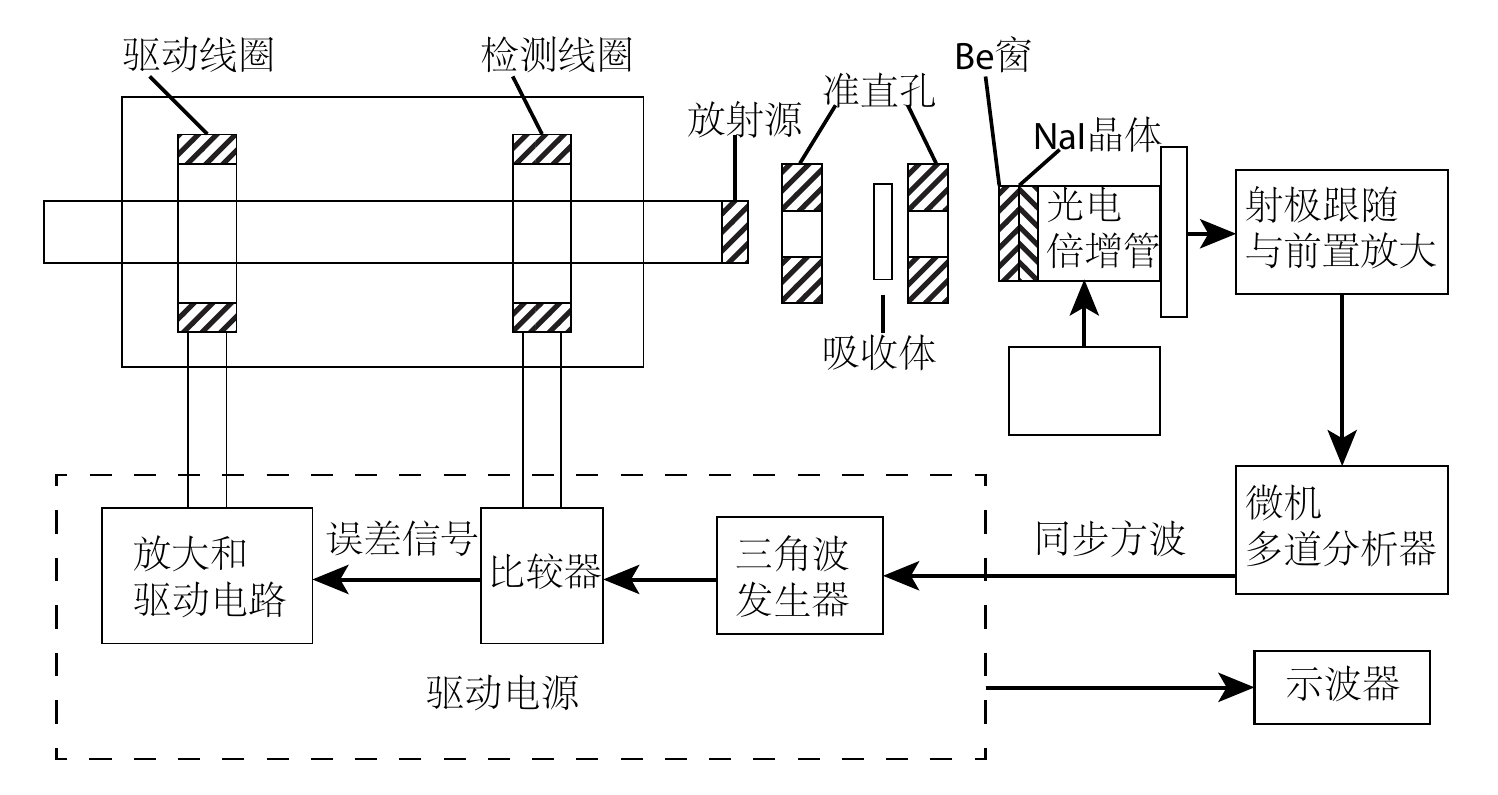
\includegraphics[width=.8\linewidth]{img/device.png}
	\caption{穆斯堡尔效应实验装置示意图,参见 \cite{textbook}. }
%	\begin{explain}
%		NULL
%	\end{explain}
	\end{figure}
\section{结果与分析}
%	实验结果应尽量以图表的形式给出. 每一个图表都应该是完整的,即阅读图表时可以不必依赖正文.\par
%	依自己意愿,实验结果和对结果的分析讨论既可分为两节也可合在一节.\par
%
%	每个图一般包含:图名、轴名、轴、刻度、标尺、数据点、曲线、图例、标注和图注等部分. 应尽量让读者不看正文就能基本理解图的含意.\par
%	逐点测量得到的函数关系要同时用表格和图给出. 需要作比较的多条曲线要画在同一图上.\par
%	为避免读者在图表和正文间反复跳跃阅读,在正文中也要对图表作必要的说明.\par
%
%	对于预料之外的实验结果,必须首先小心证明其可靠性.读者只有在相信你的实验结果时才愿意花时间看你的分析.\par
%	必须用文字归纳整理出正式的实验结果或结论.可信的实验结果是课程报告最重要的内容.作为一个实验物理工作者,分析解释出错并不丢脸,实验结果不被采信则是致命的.\par
%	教学实验的结论往往是预先知道的. 所以,教师更关心的是你的说理过程. 一般说来,单由课内实验的结果不足以能得到明确的结论. 此时,你可以引用他人的研究结果来帮助帮助自己的论证,但必须注明出处. \par
%	确实不能得到明确结论时,可以给出几种可能结论并指出可以再做哪些实验来帮助作进一步的判断.\par
%	总之,分析讨论部分要做到: 论据要valid,论证要reasonable,结论要convincing.\par
%%%%%%%%%%%%%%%%%%%%%%%%%%%%%%
	首先采集 \CoAtom 源能谱以选出所需的 \SI{14.4}{\keV} 射线,比较实验手册上 \CoAtom 源的参考能谱,可确定其中的较高峰值即对应 \SI{14.4}{\keV} $\gamma$射线。实验中估选其半高宽,并在程序上设为上、下阈值。
	\begin{figure}[!ht]
	\centering
	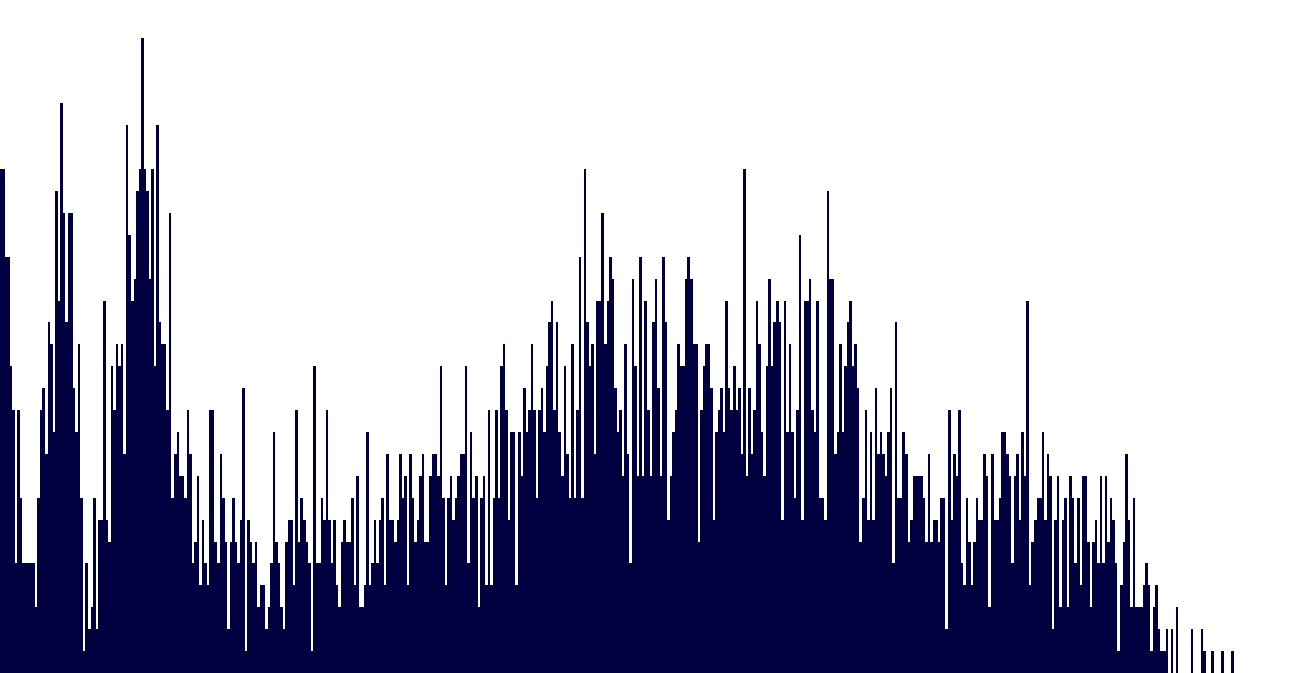
\includegraphics[
		height=8\baselineskip,
		width=.8\linewidth,
		frame
	]{data/bg_white.png}
	\caption{\CoAtom 放射源能谱图,于控制程序中截取得到。}
	\begin{explain}
		图中横轴为多道分析器的道址,正比于射线能量,共 \num{512} 道;纵轴为计数,表征相应能量处探测到的$\gamma$光子数目。能谱图上较低能量处有两处明显峰值,其中最高者即对应 \SI{14.4}{\keV}. 
	\end{explain}
	\end{figure}
\FloatBarrier
	
	在此基础上,多道分析器切换至多度定标模式,采集 \FeAlpha 和\NaSample 样品的穆斯堡尔谱(采谱时间各有$\gtrsim \SI{2}{\hour}$),结果如下:
	\begin{figure}[!ht]
	\centering
	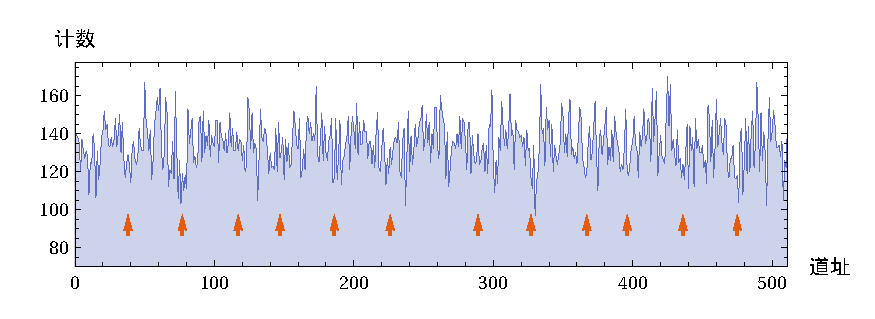
\includegraphics[width=1.\linewidth]{data/plots/feTest.pdf}
	\par
	\textit{\tup{(1)} \FeAlpha}
	\par
	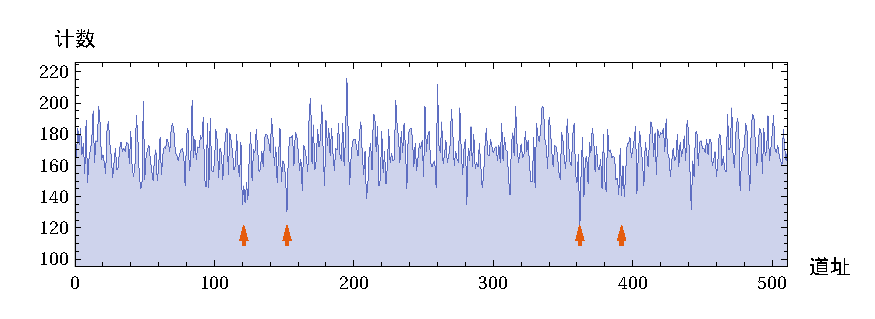
\includegraphics[width=1.\linewidth]{data/plots/naTest.pdf}
	\par
	\textit{\tup{(2)} \NaSample}
	\caption{
		所测两种样品的穆斯堡尔谱,箭头标志处为参考谱的吸收峰位置。
	}
	\end{figure}
\FloatBarrier
	
	可见,虽经$\gtrsim \SI{2}{\hour}$采谱,所得光子计数仍然很低,且难以识别出吸收峰;可见实验用信号源偏弱。事实上,\CoAtom 半衰期$\sim\SI{270}{\day}$, 数年后其强度已经过低,难以得到足够强的谱线;故此后采用参考谱进行分析。
	
	不过,若将参考谱吸收峰的位置标示于实验所得谱中,可见参考处附近确有吸收迹象,不过难以排除选择性确认偏差(confirmation bias),故此处不作为有效结果。
	
\clearpage
	\noindent 下面基于参考谱进行分析。参考谱如下:
	\begin{figure}[!ht]
	\centering
	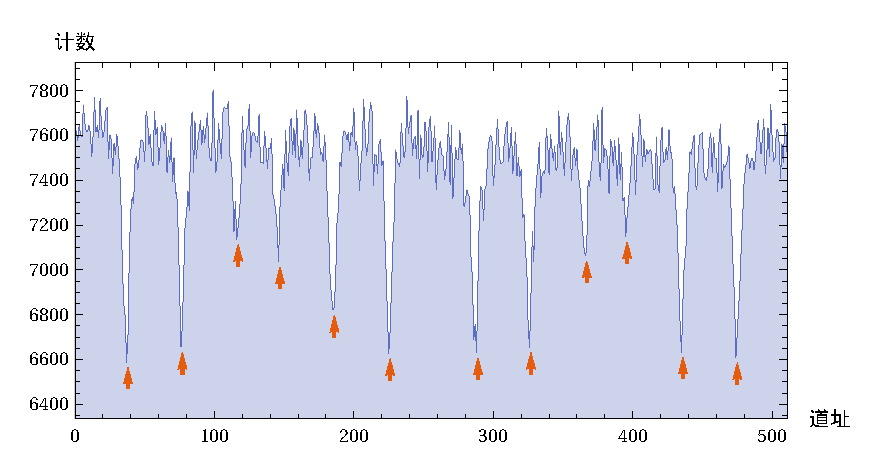
\includegraphics[width=1.\linewidth]{data/plots/feRef.pdf}
	\par
	\textit{\tup{(1)} \FeAlpha}
	\par
	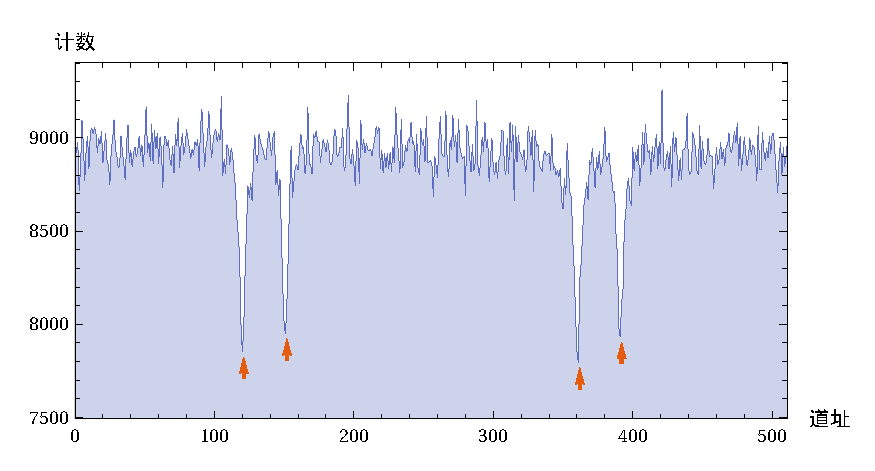
\includegraphics[width=1.\linewidth]{data/plots/naRef.pdf}
	\par
	\textit{\tup{(2)} \NaSample}
	\caption{
		所测两种样品的穆斯堡尔参考谱,箭头标志处为吸收峰位置。
	}
	\end{figure}
\FloatBarrier
\clearpage
\setlength{\jot}{0pt}
	
	可见,参考谱计数比实验所得高过一个量级,相应地吸收峰明显,适合作为定量分析。首先,具体峰值位置由 Mathematica 的 \verb|FindPeaks| 函数给出,有:
	\begin{table}[!h]
	\vspace{0\baselineskip}
	\caption[峰值道址]{参考穆斯堡尔谱的峰值道址}
	\footnotesize
	\textit{\tup{(1)} \FeAlpha}\\[1ex]
	\begin{tabularx}{.85\linewidth}{%
		C{1} | *6{C{.5}}
	}
	\toprule\midrule
		序号 &
			1 & 2 & 3 & 4 & 5 & 6 \\
	\midrule
		右侧峰道址$v_R$ &
			289 & 327 & 367 & 396 & 436 & 475 \\
		左侧峰道址$v_L$ &
			226 & 186 & 147 & 117 & 77 & 38 \\
	\midrule\bottomrule
	\end{tabularx}
	
	\vspace{.8\baselineskip}
	
	\textit{\tup{(2)} \NaSample}\\[1ex]
	\begin{tabularx}{.5\linewidth}{%
		C{1} | *6{C{.5}}
	}
	\toprule\midrule
		序号 &
			1 & 2 \\
	\midrule
		右侧峰道址$v_R$ &
			362 & 392 \\
		左侧峰道址$v_L$ &
			152 & 121 \\
	\midrule\bottomrule
	\end{tabularx}
	%\label{tab:}
	\vspace{-.3\baselineskip}
	\end{table}%
\FloatBarrier\noindent
	注意右侧峰道址随序号递增,而左侧峰递减,原因在于它们分别对应一个速度周期中的上升、下降区间。
	
	参见 \cite{textbook}, 已知 \FeAlpha 第1和第6谱线间距
		$\mcal{V} = \SI{10.656}{\mm/\s}$, 
	可得道增益:
	\begin{equation}
		K = \frac{\mcal{V}}{\abs{v_6 - v_1}}
		\simeq \SI{5.70e-2}{\mm/\s}
	\end{equation}
	其中$\abs{v_6 - v_1}$由左右道址之结果平均给出,以下类似。
	
	考虑 \FeAtom 的核塞曼分裂,可估测其发射$\gamma$射线的能量重心:
	\begin{equation}
		v_c \sim \frac{v_1 + v_2 + v_5 + v_6}{4}
		= \left\lbrace\ 
		\begin{aligned}
			&381.75, &&v\to v_R\\[-.5ex]
			&131.75, &&v\to v_L
		\end{aligned}
		\right.
	\end{equation}
	再利用 \FeAlpha 相对于源中 \FeAtom 核的同质异能移位值\supercite{textbook} $\mcal{V}' = \SI{-0.185}{\mm/\s}$, 可得该谱仪的零速度道址为:
	\begin{equation}
		v_0
		= v_c \pm \frac{\mcal{V}'}{K}
		= \left\lbrace\ 
		\begin{aligned}
			&385,   &v\to v_R\\[-.5ex]
			&128.5, &v\to v_L
		\end{aligned}
		\right.
	\end{equation}
\restorejot
\clearpage
	
	零速度道址间隔$385-128.5 = 256.5 \approx 256 = 512/2$, 表明放射源速度周期与512道基本匹配;反之,在确定速度变化与道址匹配的前提下,这一结果实质上验证了同质异能移位的存在性,并检验了$\mcal{V}'$值的可靠性。
	
	进一步,具体计算超精细结构:
	\begin{enumerate}
	\item \textbf{核塞曼分裂:}比较前述能级图与能谱图,由\supercite{textbook} $\frac{E_0}{c} = \num{4.80766e-8} \frac{\si{\eV}}{\si{\mm/\s}}$, 可得塞曼分裂裂距:
	\begin{gather}
		\Delta E_g = \frac{\abs{v_4 - v_2} + \abs{v_5 - v_3}}{2}
			\cdot \frac{K}{c}\, E_0
		\simeq \SI{1.897e-7}{\eV},\\[.5ex]
		\Delta E_e = \frac{\abs{v_3 - v_2} + \abs{v_5 - v_4}}{2}
			\cdot \frac{K}{c}\, E_0
		\simeq \SI{1.089e-7}{\eV},
	\end{gather}
	上述结果均已对$v_L, v_R$平均。考虑到 \FeAtom 内磁场\supercite{textbook} $B \simeq \SI{33}{\tesla}$, 由$\Delta E = g\mu_N B$, 以及$\mu_N \simeq \SI{3.152451e-8}{\eV/\tesla}$, 可得:
	\begin{gather}
		g_g \simeq 0.182,\quad g_e \simeq 0.105,\\
		\mu_g \simeq \SI{5.75e-9}{\eV/\tesla},\quad
		\mu_e \simeq \SI{3.30e-9}{\eV/\tesla}
	\end{gather}
	\item \textbf{同质异能移位:}\NaSample 相对 \FeAlpha 的重心偏移为:
	\begin{equation}
		\Delta v = \abs{
			\pqty{\frac{v_1 + v_2}{2}}_{
				{\text{\NaSample}}
			}
			- \pqty\Big{v_c}_{\text{\FeAlpha}}
		} = 4.75
	\end{equation}
	结合道增益$K$及零速度道址,可得相对移位 \SI{+0.271}{\mm/\s}, 对应$\Delta E = +\SI{1.30e-8}{\eV}$. 
	\item \textbf{电四极分裂:}同样,对\NaSample 样品,比较能级图,可得:
	\begin{equation}
		\Delta E = \abs{v_1 - v_2} \cdot \frac{K}{c}\, E_0
		\simeq \SI{8.36e-8}{\eV},
	\end{equation}
	此即 \FeAtom 第一激发态的电四极分裂裂距。
	\end{enumerate}
	
	此外,注意到吸收峰半高宽$\simeq \numrange{5}{6}$道,对应:
	\begin{equation}
		2\Gamma
		\gtrsim 5\times\frac{K}{c}\, E_0
		\simeq \SI{1.37e-8}{\eV}
	\end{equation}
	比激发态寿命对应的半高宽$\sim\SI{.98e-8}{\eV}$来得宽,相应地,对应寿命$\tau = \hbar/\Gamma \simeq \SI{.096}{\us}$比$\SI{.14}{\us}$来得稍短。由于源和吸收体均存在一定厚度,估计上述展宽主要源于自吸收的影响。
\section{结论}
%%%	首先要给出实验结果,然后再给出由实验结果分析得到的结果和结论。此部分给出的内容要比摘要中的全面,用词要更准确。\par
%%%%%%%%%%%%%%%%%%%%%%%%%%%%%%%
	本实验以 \CoAtom 作为$\gamma$源,利用多普勒效应微调制光子能量,获得了 \FeAlpha 和\NaSample 样品的穆斯堡尔吸收谱。在此基础上,结合已知参量校准了谱仪,进而研究了 \FeAtom 核能级的超精细结构,确定了 \FeAlpha 中 \FeAtom 的塞曼裂距、核磁矩及朗德$g$因子,测定了硝普酸钠中 \FeAtom 相对于 \FeAlpha 的同质异能移位及其电四极裂距。
	
	实验表明,将穆斯堡尔效应用于高分辨能级探测是十分强大的,尤其便于探测原子核的精超细结构。
\section{致谢}
%	此部分感谢同组人...和对实验和报告有帮助的人。
%%%%%%%%%%%%%%%%%%%%%%%%%%%%%%
	感谢张双全老师的细致指导和耐心帮助;感谢 \TeX\, - \LaTeX\, Stack Exchange\footnote{%
		\url{https://tex.stackexchange.com/}
	}, 助我解决了众多排版问题。
\clearpage

\setlength{\bibsep}{2pt}
\linespread{1.2}\selectfont
\bibliographystyle{../BibStyle/gbt-7714-2015-numerical}
\bibliography{../BibStyle/Textbook,bib/Ref}

\clearpage
\end{document}
